% !TeX root = RDT.tex
\documentclass[a4paper, 11pt]{article}    

\usepackage[ngerman]{babel}                   
\usepackage[onehalfspacing]{setspace}
\usepackage[top=2.5cm,bottom=2.5cm,left=2cm,right=2cm,marginparwidth=1.75cm]{geometry}

% Load useful packages                        
\usepackage{amsmath}                            
\usepackage{xcolor}                             
\definecolor{custom-blue}{RGB}{0,99,166} 
\usepackage{hyperref}
\hypersetup{colorlinks=true, allcolors=custom-blue}
\usepackage[default]{sourcesanspro}             
\usepackage[T1]{fontenc}                        
\usepackage{wrapfig}
\usepackage{fancyhdr}
\usepackage{longtable}
\usepackage{lastpage}
\usepackage{float}
\usepackage{tabularx} 
\usepackage[normalem]{ulem}
\useunder{\uline}{\ul}{}
\usepackage{booktabs}
\usepackage{graphicx}
\usepackage{color}
\usepackage{tabularray}
\usepackage{enumitem}
\usepackage{subcaption}


\pagestyle{myheadings}
\pagestyle{fancy}     

\definecolor{Alto}{rgb}{0.878,0.878,0.878}
\definecolor{Nobel}{rgb}{0.701,0.701,0.701}

\setlength{\headheight}{30pt}
\renewcommand{\headrulewidth}{0.5pt}
\renewcommand{\footrulewidth}{0.5pt}

\fancyhead[C]{}                                 
\fancyhead[R]{}                      
\fancyfoot[L]{}
\fancyfoot[C]{}                 
\fancyfoot[R]{\thepage/\pageref{LastPage}}

\title{
    MHS3D
}

\begin{document}

\maketitle
\clearpage

\tableofcontents
\clearpage

%
\section{Requirements}
\begin{enumerate}
    \item Die Smartwatch soll den MPU6050 Beschleunigungssensor + Gyroskop ansteuern und deren Messdaten abfragen können.
    \item Die von der Uhr gesammelten Messdaten sollen im laufenden Betrieb an einen PC übertragen werden können.
    \item Bewegungsrichtungen sollen live in 3D (als Linie im “Raum”) angezeigt werden.
    \item Das Bewegungstracking der letzten 2 Stunden soll während des Betriebs gespeichert und dargestellt werden können.

\end{enumerate}

Erweiterungsideen:
\begin{itemize}
    \item Der Puls des Trägers  wird als Liniendiagramm, gefärbt nach Bereichen, altersabhängig (grün bis rot) angezeigt werden.
    \item Pulsänderungen sollen als farbliche Veränderung des Bewegungsstriches im Raum visualisiert werden.
    \item Aufnahme der Daten in Sessions mit Button an der Uhr als Start/Stop
    \item Interaktive Drehung der Ansicht möglich
    \item Mapping der Bewegungen in die Raumpläne der HAW
\end{itemize}
\clearpage


\section{Projektplan}
\subsection{Projektaufbau}
Ein Projektplan der bei Konkretisierung und Arbeitsteilung nach dem Aufstellen der Anforderungen entstanden ist.

\begin{figure}[H]
    \centering
    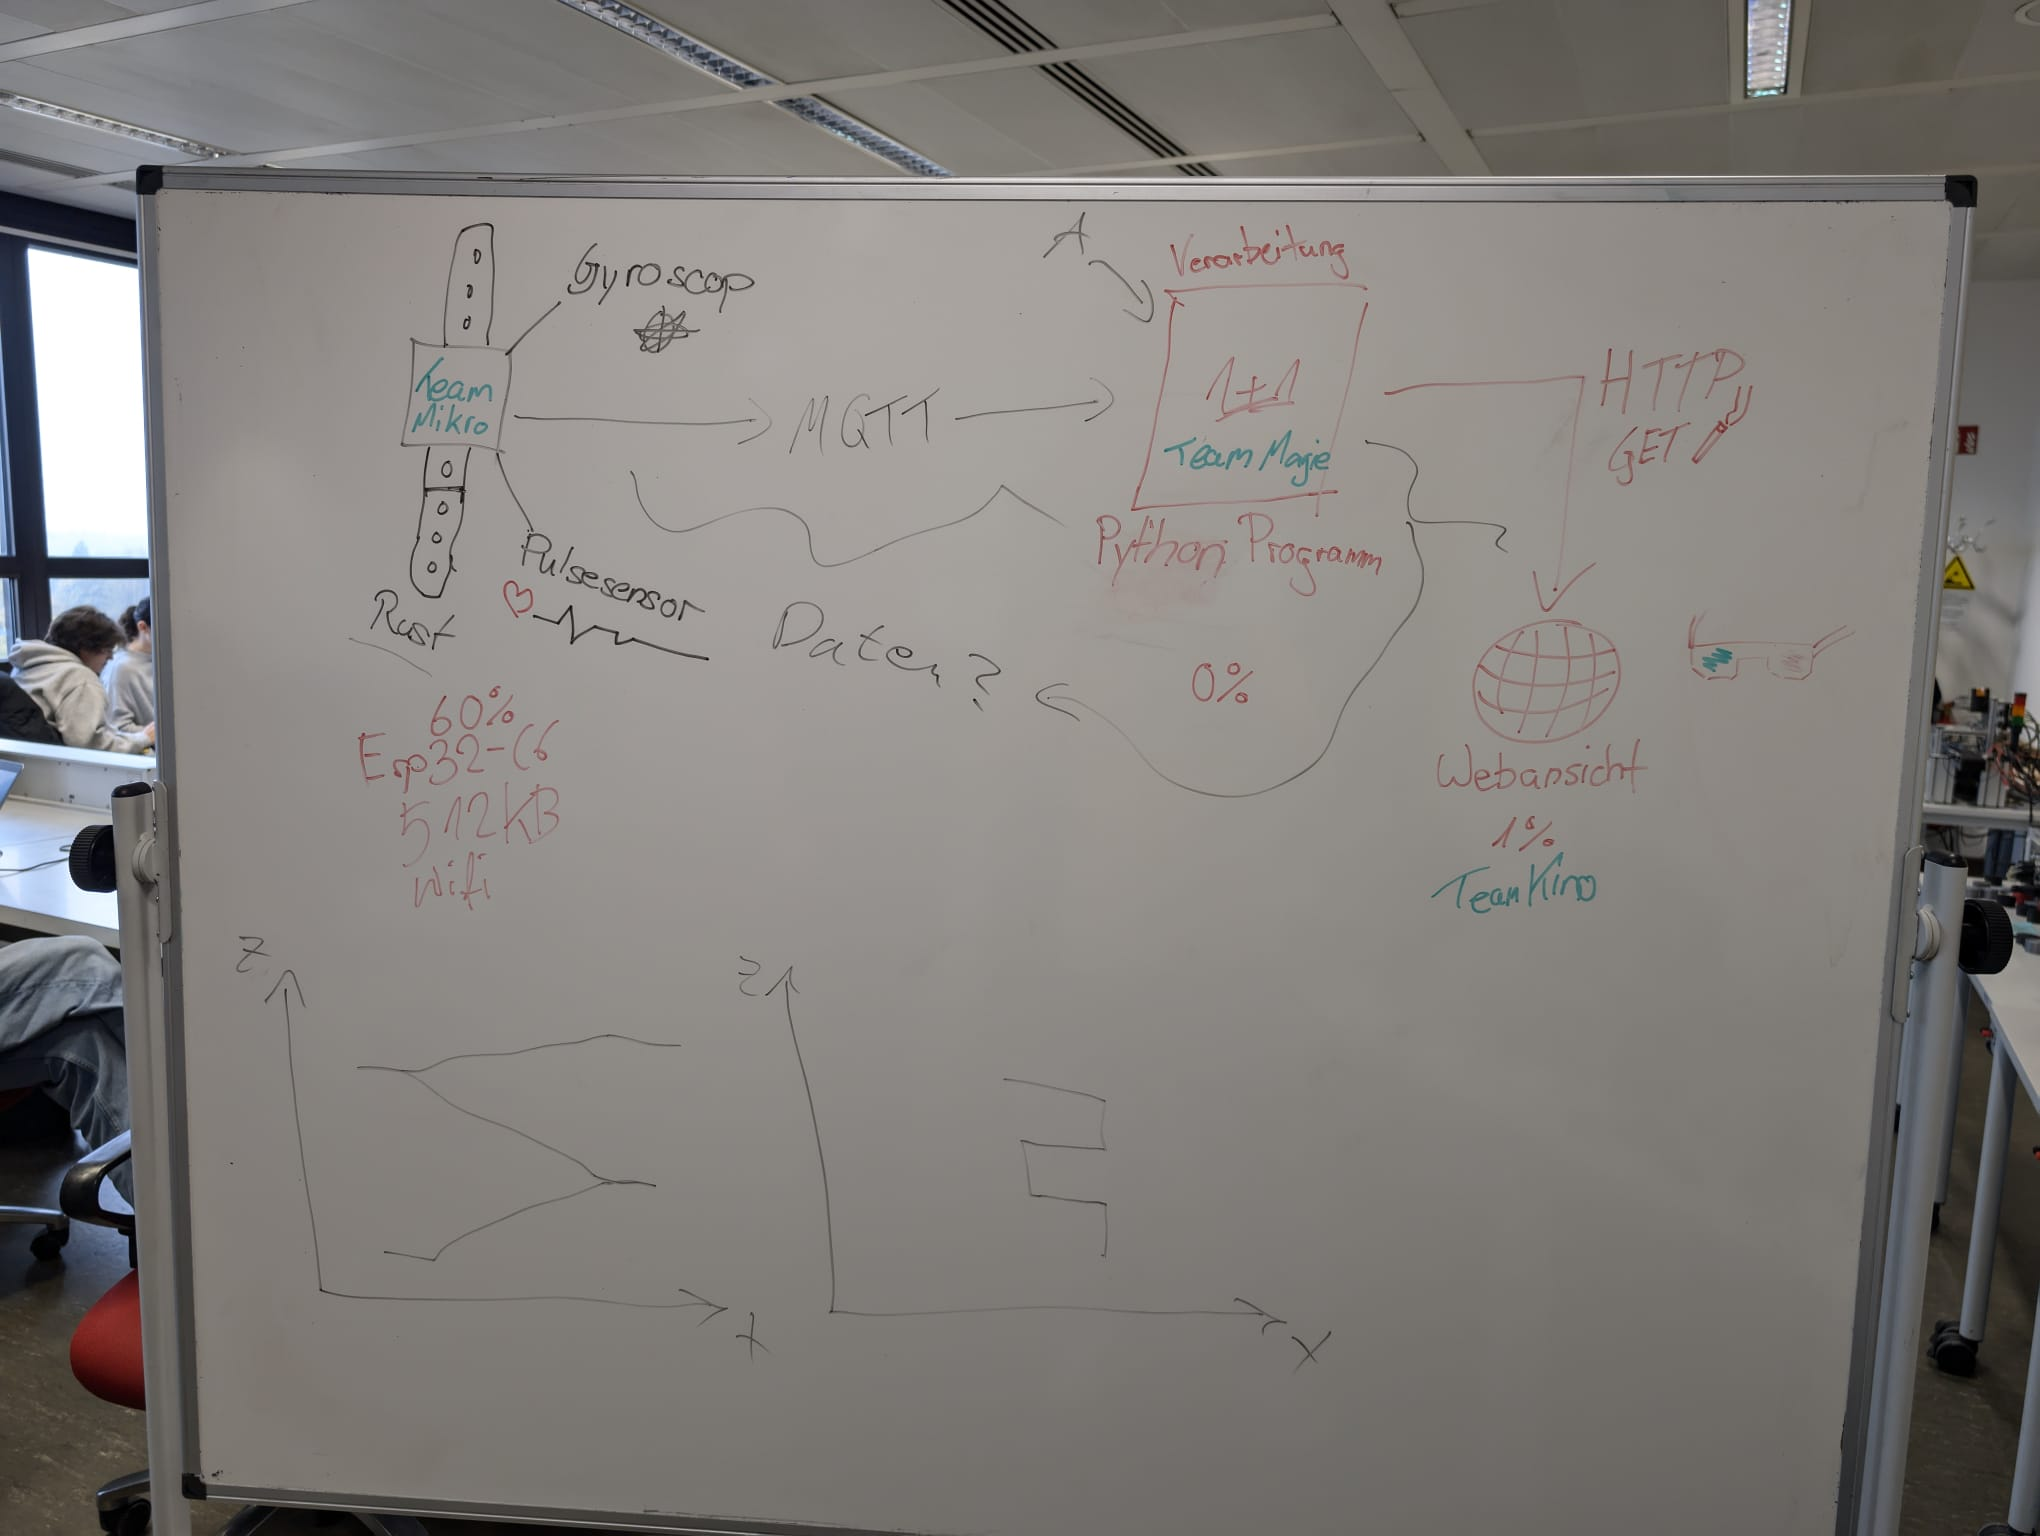
\includegraphics[width=0.7\textwidth]{images/Projektaufbau.jpeg}
    \caption{Projektaufbau}
    \label{fig:Projektaufbau}
\end{figure}
\noindent Die Idee war es mit der Uhr über die Sensorik Daten zu sammeln, diese per MQTT einem PC/Laptop zur Verfügung zu stellen und dort die gesammelten Daten aufzubereiten um diese dann in einer Webansicht darstellen zu können.

\noindent Nach der Gruppeneinteilung haben wir uns entschieden den Code für die Uhr in Rust zu schreiben, die Datenaufbereitung in Python zu machen und diese Daten per HTTP einem Javaprogramm zur Darstellung zugänglich zu machen.

\noindent (vermutlich um angepassten digitalen Projektaufbau ergänzen/ersetzen und Änderungsgründe erläutern)


\clearpage
\subsection{grober Zeitplan}
Ein grober Zeitplan der Recherche und Umsetzung des Projektplans den wir zu Anfang der Planung geschrieben haben.
\begin{center}
    \begin{tabularx}{\textwidth}{ |c|X|X|X| }
        \hline
        \textbf{KW} & \textbf{Micro}                                    & \textbf{Magic}        & \textbf{Kino}                            \\
        \hline
        \textbf{44} & Projekt aufsetzen                                 &                       &                                          \\
        \hline
        45          & Daten per HTTP senden, Format der Daten festlegen & Recherche Algorithmen & Recherche: Darstellung Was und Wie?      \\
        \hline
        \textbf{46} &                                                   &                       & Mockups erstellen                        \\
        \hline
        47          & Herzschrittzähler zum Laufen kriegen              &                       & Aufsetzen des Frontends                  \\
        \hline
        \textbf{48} & Done                                              &                       &                                          \\
        \hline
        49          &                                                   &                       & Testen der Darstellung mit Dummy-Daten   \\
        \hline
        \textbf{50} &                                                   &                       &                                          \\
        \hline
        51          &                                                   &                       & Daten von Magic empfangen und darstellen \\
        \hline
        \textbf{54} &                                                   &                       &                                          \\
        \hline
        55          &                                                   &                       & Testen                                   \\
        \hline
        \textbf{56} &                                                   &                       &                                          \\
        \hline
        57          &                                                   &                       &                                          \\
        \hline
    \end{tabularx}
\end{center}
\clearpage

\section{Schaltplan}
\begin{figure}[H]
    \centering
    \begin{subfigure}{0.64\textwidth}
        \centering
        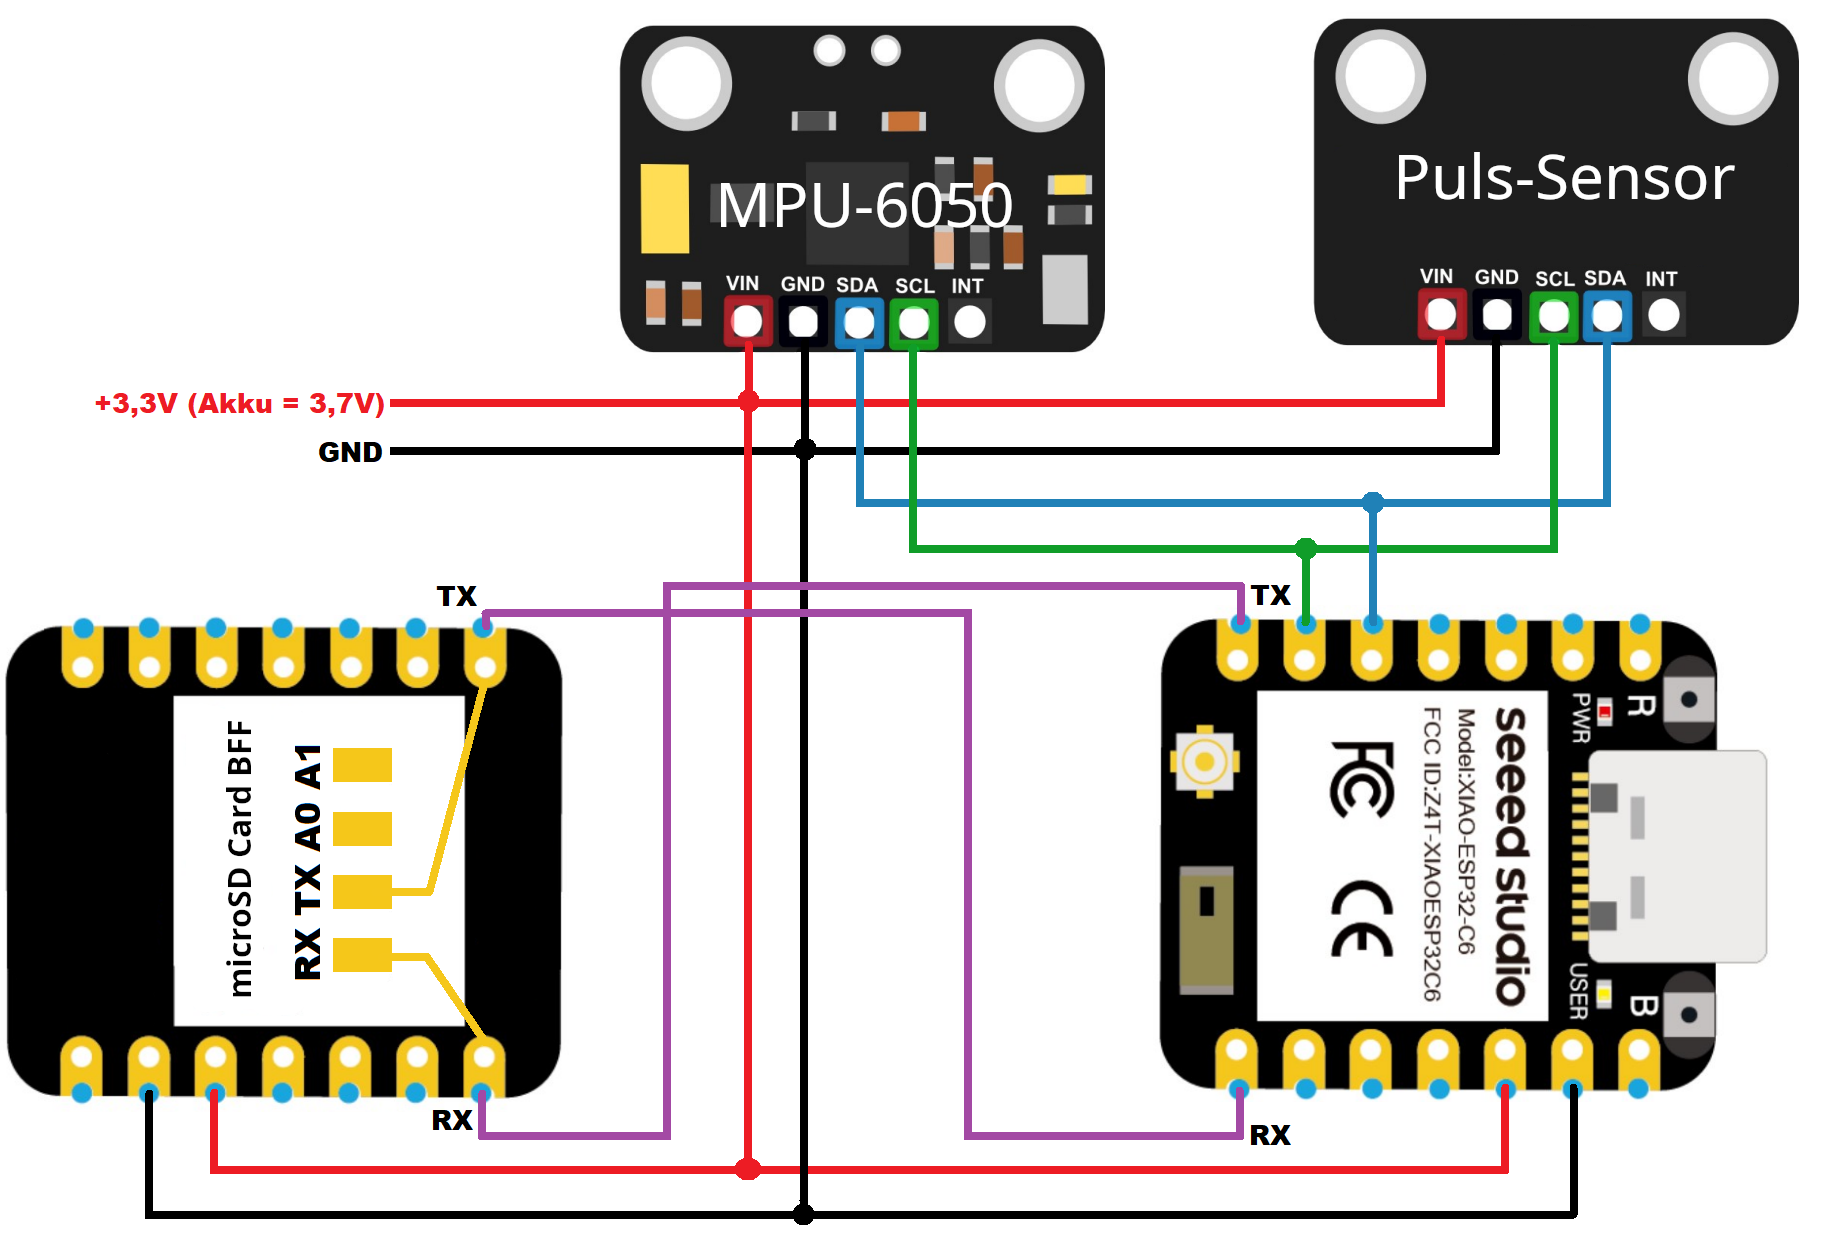
\includegraphics[width=\textwidth]{images/Schaltplan_v1.png}
        \caption{Schaltplan Smartwatch}
        \label{fig:Schaltplan Smartwatch}
    \end{subfigure}
    \begin{subfigure}{0.34\textwidth}
        \centering
        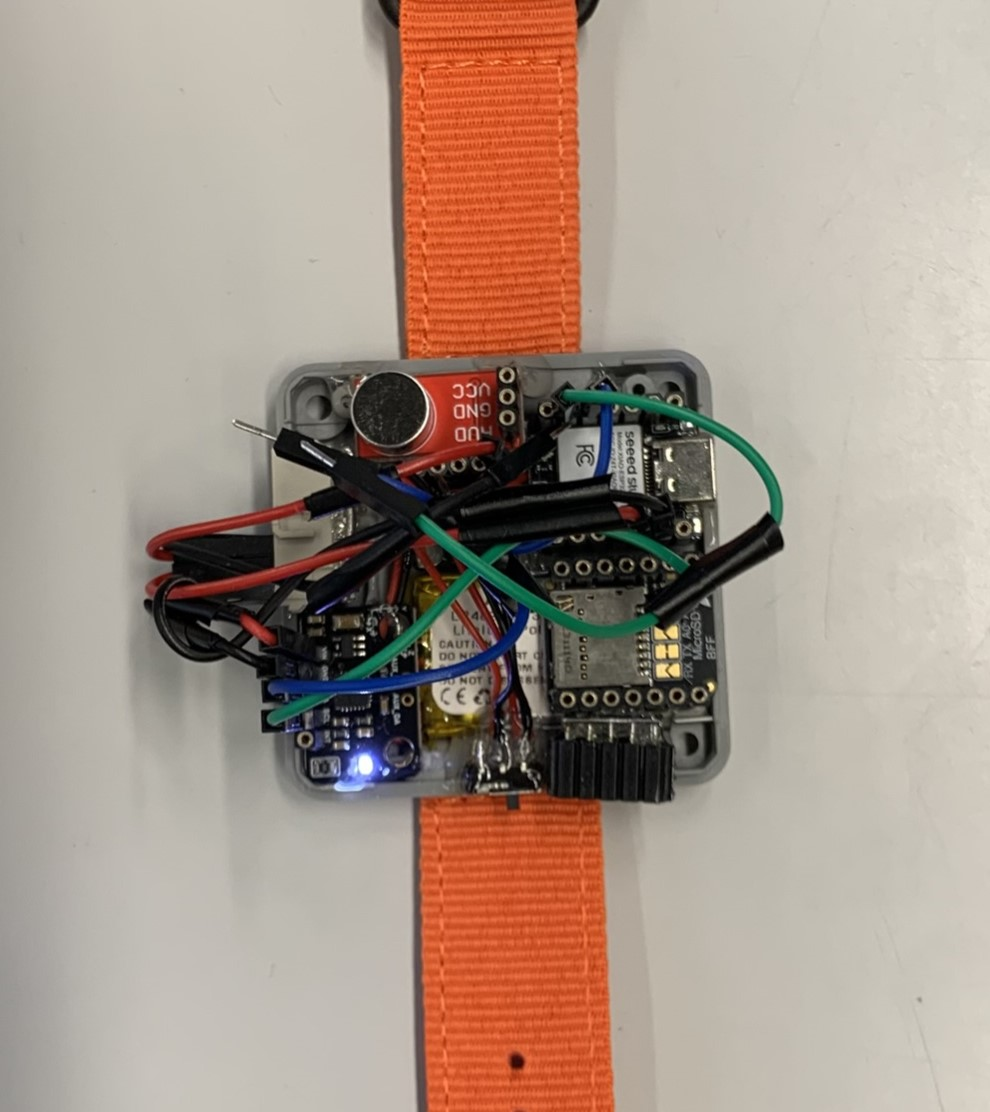
\includegraphics[width=\textwidth]{images/verkabelte_Smartwatch_cropped.JPEG}
        \caption{verkabelte Smartwatch}
        \label{fig:verkabelte Smartwatch}
    \end{subfigure}
\end{figure}
An den Mikrocontroller haben wir einen Puls-Sensor, den MPU-6050, ein 3-Achsen Gyroskop und Beschleunigungssensor, sowie einen microSD Kartenslot angeschlossen.

\noindent Zur Stromversorgung haben wir die Sensoren, den microSD Kartenslot und den Mikrocontroller mit 3,3V + Ground (im Schaltplan Rot + Schwarz) verbunden, zur Kommunikation zwischen dem Mikrokontroller und dem Puls-Sensor und dem MPU-6050 benutzen wir I2C (im Schaltplan Grün und Blau).

\noindent Die microSD Karte ist für lesende und schreibende Kommunikation mit 2 Rx Tx Verbindungen an den Mikrocontroller angeschlossen (im Schaltplan Lila).

\noindent Zur vereinfachten Verkabelung sind zwei Steckleisten auf der Uhr befestigt über die einmal die Stromversorgung und einmal die I2C Kabel gesteckt wurden.

\subsection{Stromverbrauch der Uhr:}
der Akku umfasst 700 mAh, der MPU6050 benötigt 4 mA  und der ESP32C6 im Worst Case 240mA da wir wlan für http benötigen.
Daraus ergibt sich bei unserer Verwendung für die Uhr eine Laufzeit von 2,8h.

\clearpage

\section{Datenübertragung}
Die Datenübertragung findet als HTTP GET Anfrage an den Webserver der Smartwatch statt. Die Smartwatch liefert dann einen JSON String von Datensätzen.

\noindent
Ein Datensatz enthält einen Timestamp, Acceleration x,y und z Achse, Gyroskop x,y und z Achse sowie ein Pulssensor Messwert in Folgendem Format:

\clearpage

\end{document}